
\begin{center}

\includegraphics[width=0.7\textwidth]{content/3/chapter4/images/2.png}\\
\end{center}

为了充分理解概念,先从概念出现原因说起。

\subsubsubsection{4.1.1\hspace{0.2cm}两种错误的方法}

C++20之前,可以有两种截然相反的方式来考虑函数或类:为特定类型或为泛型类型定义它们。后者,称之为函数模板或类模板。这两种方法都有各自的问题:

\hspace*{\fill} \\ %插入空行
\noindent
\textbf{4.1.1.1\hspace{0.2cm}太具体}

为每种类型重载函数或重新实现类是一项乏味的工作。为了避免这种重复,类型转换通常是我们的救星。不过,看似拯救,却又是诅咒。

\hspace*{\fill} \\ %插入空行
\noindent
\textbf{类型的隐式转换}
\begin{lstlisting}[style=styleCXX]
// tooSpecific.cpp

#include <iostream>

void needInt(int i){
	std::cout << "int: " << i << '\n';
}

int main(){

	std::cout << std::boolalpha << '\n';
	
	double d{1.234};
	std::cout << "double: " << d << '\n';
	needInt(d);
	
	std::cout << '\n';
	
	bool b{true};
	std::cout << "bool: " << b << '\n';
	needInt(b);
	
	std::cout << '\n';

}
\end{lstlisting}

例子中(第13行),我以double开始,以int结束(第15行)。第二次,我以bool开始(第19行),并以int结束(第21行)。

\begin{center}
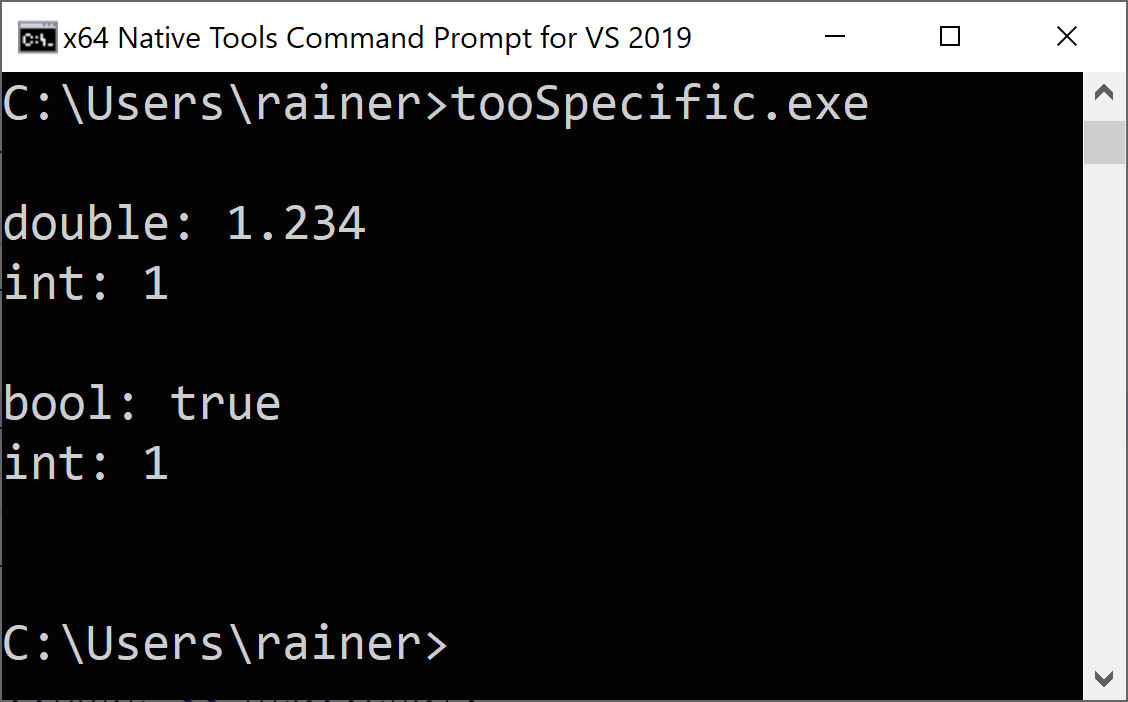
\includegraphics[width=0.6\textwidth]{content/3/chapter4/images/3.png}\\
类型的隐式转换
\end{center}

程序进行了两次隐式的类型转换。

\hspace*{\fill} \\ %插入空行
\noindent
\textbf{4.1.1.1.1\hspace{0.2cm}窄化转换}

使用double类型调用getInt(int a)可以实现窄化转换。窄化转换是一种类型转换,包括精度损失。我猜有时你并不想有任何损失。

\hspace*{\fill} \\ %插入空行
\noindent
\textbf{4.1.1.1.2\hspace{0.2cm}类型提升}

反过会更好吗?

使用bool类型调用getInt(int a)将bool类型提升为int类型。惊讶吗?许多C++开发人员在添加两个bool时,并不知道他们会得到的是哪种数据类型。

\hspace*{\fill} \\ %插入空行
\noindent
\textbf{对两个布尔值进行加法运算}
\begin{lstlisting}[style=styleCXX]
template <typename T>
auto add(T first, T second){
	return first + second;
}

int main(){
	add(true, false);
}
\end{lstlisting}

\href{https://cppinsights.io/s/9bd14f99}{C++ Insights}在编译器在实例化中转换函数模板后,并将上面的源代码可视化。

\begin{lstlisting}[style=styleCXX]
template <typename T>
auto add(T first, T second){
	return first + second;
}

int main(){
	add(true, false);
}
\end{lstlisting}

\begin{center}
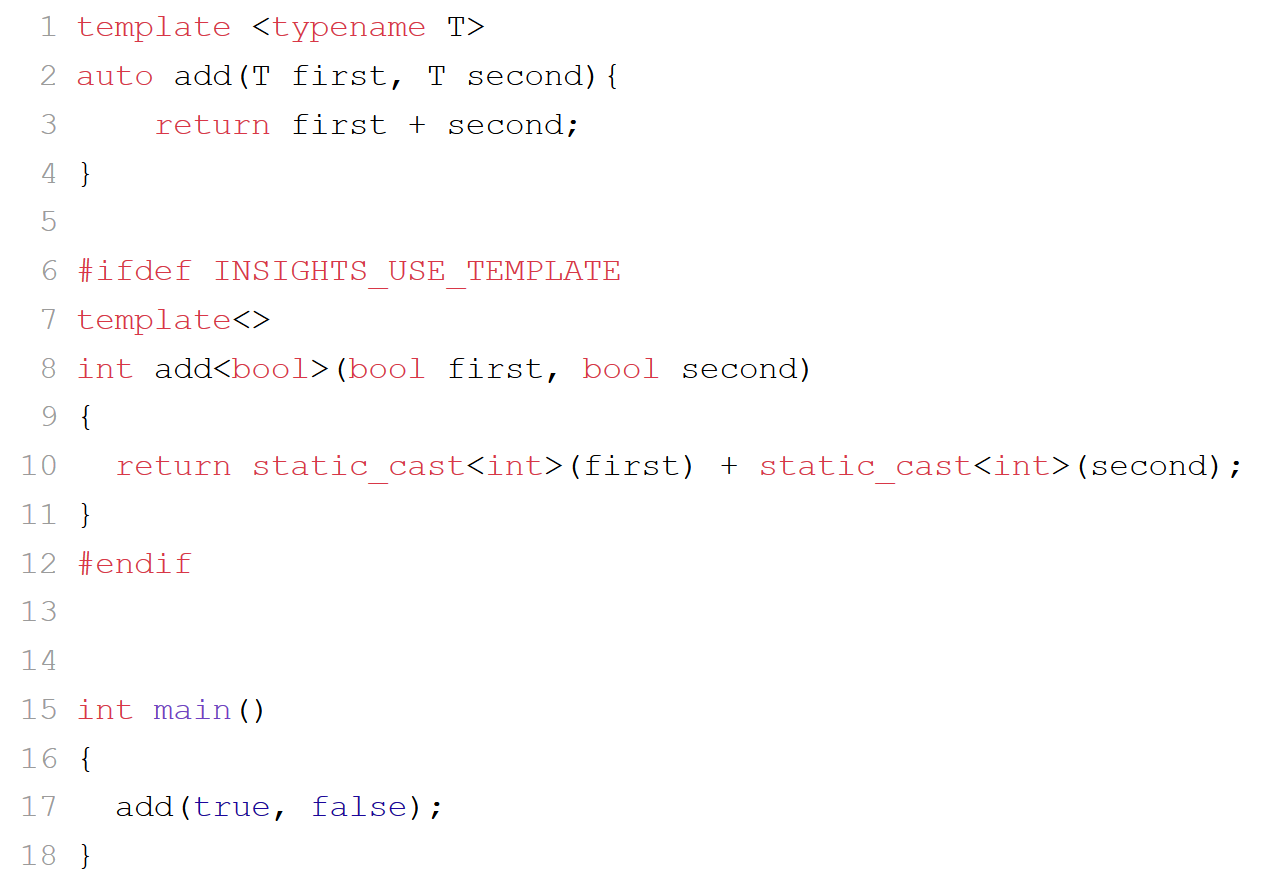
\includegraphics[width=0.8\textwidth]{content/3/chapter4/images/1-1.png}\\
bool提升为int
\end{center}

第8-14行是\href{https://cppinsights.io/}{C++ Insights}截图中的关键行。函数模板add的模板实例化,使用返回类型int创建一个完整的特化。两个bool都隐式提升为int。

为了方便起见,我们依赖于转换的魔力,因为我们不想为每种类型重载函数或重新实现类。

让我试试另一种方法,用一个泛型函数。这能拯救我们吗?

\hspace*{\fill} \\ %插入空行
\noindent
\textbf{4.1.1.2\hspace{0.2cm}太通用}

Sorting a container is a general idea. It should work for each container if its elements support ordering. In the following example, I apply the standard algorithm std::sort to the standard container std::list.

\hspace*{\fill} \\ %插入空行
\noindent
Sorting a std::list
\begin{lstlisting}[style=styleCXX]
// tooGeneric.cpp

#include <algorithm>
#include <list>

int main(){
	
	std::list<int> myList{1, 10, 3, 2, 5};
	
	std::sort(myList.begin(), myList.end());
	
}
\end{lstlisting}

\begin{center}
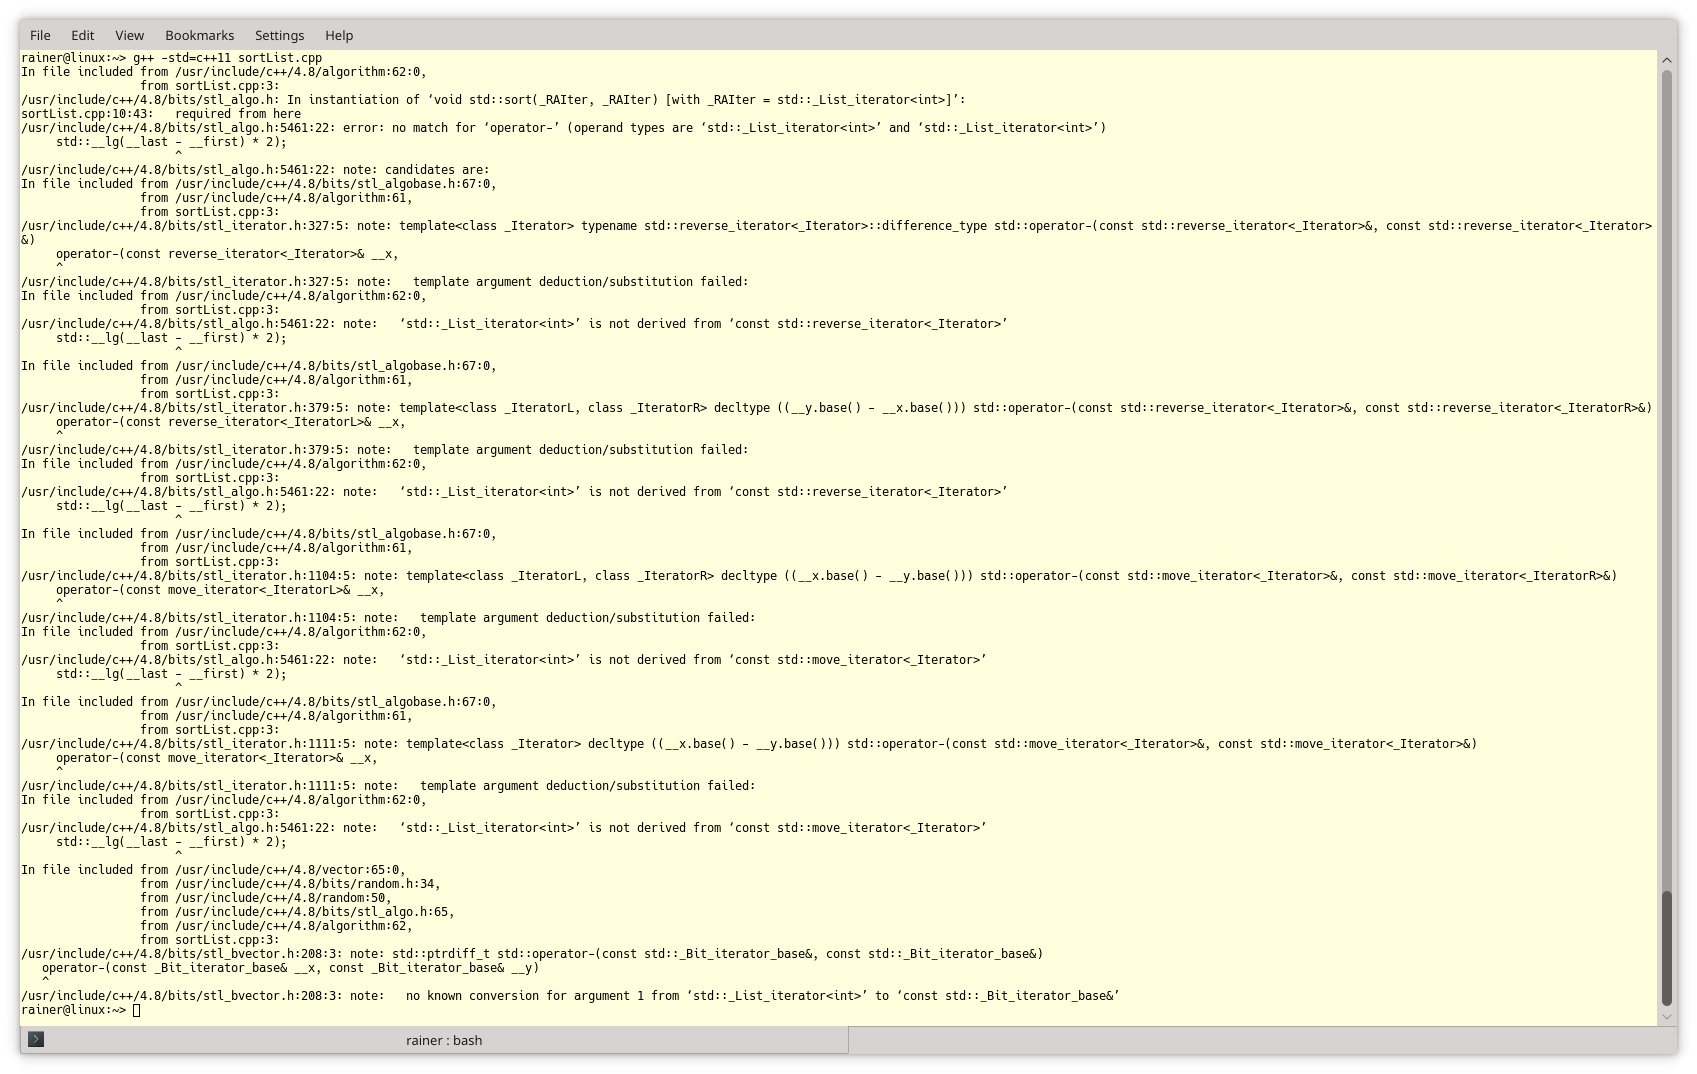
\includegraphics[width=1.0\textwidth]{content/3/chapter4/images/4.png}\\
A compiler error when trying to sort a std::list
\end{center}

I don’t even want to decipher this long message. What’s gone wrong? Let’s take a look at the signature of the specific overload of \href{https://en.cppreference.com/w/cpp/algorithm/sort}{std::sort} used in this example.

\hspace*{\fill} \\ %插入空行
\begin{lstlisting}[style=styleCXX]
template< class RandomIt >
constexpr void sort( RandomIt first, RandomIt last );
\end{lstlisting}

std::sort uses strange-named argument types such as RandomIt. RandomIt stands for a randomaccess iterator and gives the key hint for the overwhelming error message. A std::list only provides a bidirectional iterator, but std:sort requires a random-access iterator. The following graphic shows why a std::list does not support a random access iterator.

\begin{center}

\includegraphics[width=0.5\textwidth]{content/3/chapter4/images/5.png}\\
\end{center}

If you study the std::sort documentation on cppreference.com, you will find something exciting: type requirements on template parameters. They place conceptual requirements on the types that have been formalized into the C++20 feature, concepts.

\noindent
4.1.1.3\hspace{0.2cm}拯救概念

Concepts put semantic constraints on template parameters. std::sort has overloads that accept a comparator.

\begin{lstlisting}[style=styleCXX]
template< class RandomIt, class Compare >
constexpr void sort(RandomIt first, RandomIt last, Compare comp);
\end{lstlisting}

These are the type requirements for the more powerful overload of std::sort:

\begin{itemize}
\item 
RandomIt must meet the requirements of ValueSwappable and LegacyRandomAccessIterator

\item 
The type of the dereferenced RandomIt must meet the requirements of MoveAssignable and MoveConstructible.

\item 
The type of the dereferenced RandomIt must meet the requirements of Compare.
\end{itemize}

Requirements such as ValueSwappable or LegacyRandomAccessIterator are so-called named requirements. Some of these requirements are formalized in C++20 in \href{https://en.cppreference.com/w/cpp/language/constraints}{concepts}.

In particular, std::sort requires a LegacyRandomAccessIterator. Let’s have a closer look at the named requirement LegacyRandomAccessIterator that is called random\_access\_iterator (part of <iterator>) in C++20:

\hspace*{\fill} \\ %插入空行
\noindent
std::random\_access\_iterator
\begin{lstlisting}[style=styleCXX]
template<class I>
	concept random_access_iterator =
		bidirectional_iterator<I> &&
		derived_from<ITER_CONCEPT(I), random_access_iterator_tag> &&
		totally_ordered<I> &&
		sized_sentinel_for<I, I> &&
		requires(I i, const I j, const iter_difference_t<I> n) {
			{ i += n } -> same_as<I&>;
			{ j + n } -> same_as<I>;
			{ n + j } -> same_as<I>;
			{ i -= n } -> same_as<I&>;
			{ j - n } -> same_as<I>;
			{ j[n] } -> same_as<iter_reference_t<I>>;
		};
\end{lstlisting}

A type I supports the concept random\_access\_iterator if it supports the concept bidirectional\_iterator and all the following requirements. For example, the requirement { i += n } -> same\_as<I\&> as part of the requires expression means that for a value of type I, { i += n } is a valid expression, and it returns a value of type I\&. To complete the sorting story, std::list does support a bidirectional\_iterator, and not a random\_access\_iterator that std::sort requires.

When you now use an algorithm that requires a random\_access\_iterator, but you only provide a birectional\_iterator, you get a concise and readable error message saying that your iterator does not satisfy the concept random\_access\_iterator.

\begin{center}
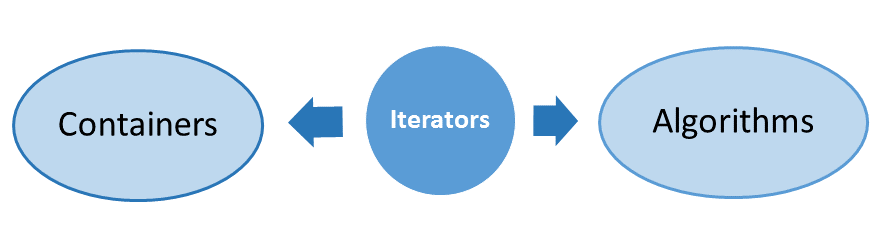
\includegraphics[width=0.5\textwidth]{content/3/chapter4/images/6.png}\\
The Standard Template Library
\end{center}

\begin{tcolorbox}[colback=blue!5!white,colframe=blue!75!black,title={泛型编程的本质}]
I want to start this short historical detour with a quote from the invaluable book \href{https://www.fm2gp.com/}{From Mathematics to Generic Programming}, written by Alexander Stepanov (creator of the Standard Template Library) and Daniel Rose (information retrieval researcher): “The essence of generic programming lies in the idea of concepts. A concept is a way of describing a family of related object types.” These related object types can be integral types such as bool, char, or int. A concept embodies a set of requirements on related types such as their supported operations, semantics, and time and space complexity.

The Standard Template Library (STL) as a generic library is based on concepts. From a bird’seye view, the STL consists of three components. Those are containers, algorithms that run on containers, and iterators that connect both of them.

Each container provides iterators that respect its structure, and the algorithms operate on these iterators. A container, such as a sequence container or an associative container, models a semi-open range. Access to the container’s elements is provided through iterators, as well as iterating through them, and the equality comparison of them. The abstraction of the STL is based on concepts such as semi-open range and iterator and allow for transparent use of the containers and algorithms of the STL.
\end{tcolorbox}

More generally, what are the advantages of concepts?

\subsubsubsection{4.1.2\hspace{0.2cm} Advantages of Concepts}

\begin{itemize}
\item 
Requirements for template parameters are part of the interface.

\item 
The overloading of functions and specialization of class templates can be based on concepts.

\item 
Concepts can be used for function templates, class templates, and generic member functions of classes or class templates.

\item 
You get improved error messages because the compiler compares the requirements of the template parameters with the given template arguments.

\item 
You can use predefined concepts or define your own.

\item 
The usage of auto and concepts is unified. Instead of auto, you can use a concept.

\item 
If a function declaration uses a concept, it automatically becomes a function template. Writing function templates is, therefore, as easy as writing a function.
\end{itemize}


\subsubsubsection{4.1.3\hspace{0.2cm} The long, long History}

The first time I heard about concepts was around 2005 - 2006. They reminded me of Haskell type classes. Type classes in Haskell are interfaces for similar types. Here is a part of \href{https://en.wikipedia.org/wiki/Haskell_(programming_language)}{Haskell’s} type classes hierarchy.

\begin{center}
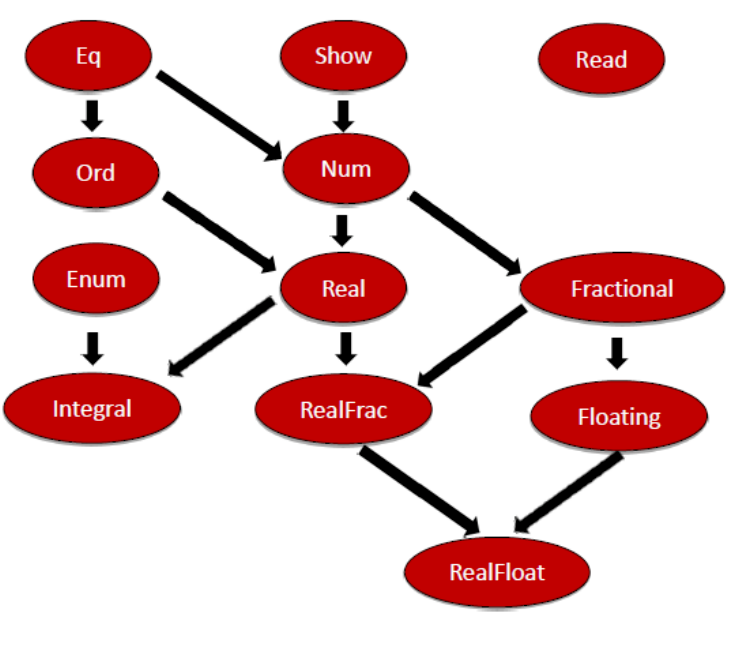
\includegraphics[width=0.8\textwidth]{content/3/chapter4/images/7.png}\\
Haskell Type Classes Hierarchy
\end{center}

But C++ concepts are different. Here are a few observations.

\begin{itemize}
\item 
In Haskell, any type has to be an instance of a type class. In C++20, a type has to fulfill the requirements of a concept.

\item 
Concepts can be used on non-type arguments of templates in C++. For example, numbers such as the value 5 are non-type arguments. For example, when you want to have a std::array of ints with 5 elements, you use the non-type argument 5: std::array<int, 5> myArray .

\item 
Concepts add no run-time costs.
\end{itemize}

Originally, concepts were going to be the key feature of C++11, but they were removed during a standardization meeting in July 2009 in Frankfurt. The quote from Bjarne Stroustrup speaks for itself: \href{https://isocpp.org/blog/2013/02/concepts-lite-constraining-templates-with-predicates-andrew-sutton-bjarne-s}{“The C++0x concept design evolved into a monster of complexity.”}. A few years later, the next try was also not successful: concepts lite were removed from the C++17 standard. They finally become part of C++20.

\subsubsubsection{4.1.4\hspace{0.2cm} Use of Concepts}

Essentially, there are four ways to use a concept.

\noindent
4.1.4.1\hspace{0.2cm} Four Ways to use a Concept

I apply the predefined concept std::integral in the program conceptsIntegralVariations.cpp in all four ways.

\hspace*{\fill} \\ %插入空行
\noindent
Four variations using the concept std::integral
\begin{lstlisting}[style=styleCXX]
// conceptsIntegralVariations.cpp

#include <concepts>
#include <iostream>

template<typename T>
requires std::integral<T>
auto gcd(T a, T b) {
	if( b == 0 ) return a;
	else return gcd(b, a % b);
}

template<typename T>
auto gcd1(T a, T b) requires std::integral<T> {
	if( b == 0 ) return a;
	else return gcd1(b, a % b);
}

template<std::integral T>
auto gcd2(T a, T b) {
	if( b == 0 ) return a;
	else return gcd2(b, a % b);
}

auto gcd3(std::integral auto a, std::integral auto b) {
	if( b == 0 ) return a;
	else return gcd3(b, a % b);
}

int main(){

	std::cout << '\n';
	
	std::cout << "gcd(100, 10)= " << gcd(100, 10) << '\n';
	std::cout << "gcd1(100, 10)= " << gcd1(100, 10) << '\n';
	std::cout << "gcd2(100, 10)= " << gcd2(100, 10) << '\n';
	std::cout << "gcd3(100, 10)= " << gcd3(100, 10) << '\n';
	
	std::cout << '\n';

}
\end{lstlisting}

Thanks to the header <concepts> in line 3, I can use the concept std::integral. The concept is fulfilled if T is the type \href{https://en.cppreference.com/w/cpp/types/is_integral}{integral}. The function name gcd stands for the greatest-common-divisor algorithm based on the \href{https://en.wikipedia.org/wiki/Euclid}{Euclidean} algorithm.

Here are the four ways to use concepts:

\begin{itemize}
\item 
Requires clause (line 6)

\item 
Trailing requires clause (line 13)

\item 
Constrained template parameter (line 19)

\item 
Abbreviated function template (line 25)
\end{itemize}

For simplicity reasons, each function template returns just auto. There is a semantic difference between the function templates gcd, gcd1, gcd2, and the function gcd3. In the case of gcd, gcd1, or gcd2, the arguments a and b must have the same type. This does not hold for the function gcd3. Parameters a and b can have different types, but must both fulfil the concept integral.

\begin{tcblisting}{commandshell={}}
gcd(100, 10) = 10
gcd1(100, 10) = 10
gcd2(100, 10) = 10
gcd3(100, 10) = 10
\end{tcblisting}

\begin{center}
Use of the concept std::integral
\end{center}

The functions gcd and gcd1 use requires clauses. Requires clauses are more powerful than you may think. Let me discuss more details to requires clauses.

\noindent
4.1.4.2\hspace{0.2cm} Requires Clause

The previous program, conceptsIntegralVariations.cpp, exemplifies that you can use a concept to define a function or function template. Of course, there are more use cases. For completeness, I want to add that you can specify the return type of a function or a function template using concepts.

The keyword requires introduces a requires clause which specifies constraints on a template argument (gcd) or on a function declaration (gcd1). requires must be followed by a compile-time predicate such as a named concept (gcd), a conjunction/disjunction of named concepts, or a requires expression.

The compile-time predicate can also be an expression:

\hspace*{\fill} \\ %插入空行
\noindent
Using a compile-time predicate in a requires clause
\begin{lstlisting}[style=styleCXX]
// requiresClause.cpp

#include <iostream>

template <unsigned int i>
requires (i <= 20)
int sum(int j) {
	return i + j;
}


int main() {

	std::cout << '\n';
	
	std::cout << "sum<20>(2000): " << sum<20>(2000) << '\n',
	// std::cout << "sum<23>(2000): " << sum<23>(2000) << '\n', // ERROR
	
	std::cout << '\n';

}
\end{lstlisting}

The compile-time predicate used in line 6 exemplifies an interesting point: the requirement is applied on the non-type i, and not on a type as usual.

\begin{tcblisting}{commandshell={}}
sum<20>(2000): 2020
\end{tcblisting}

\begin{center}
Compile-time predicates in a requires clause
\end{center}

When you use line 17, the clang compiler reports the following error:

\begin{center}
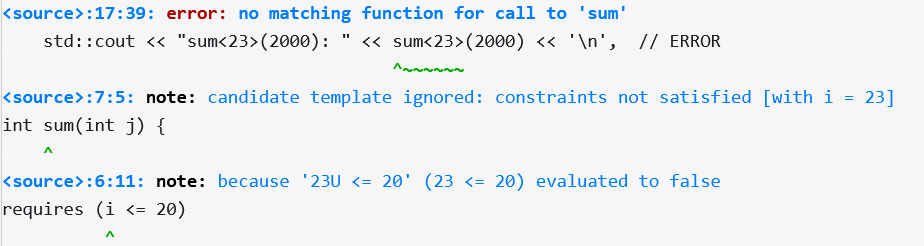
\includegraphics[width=1.0\textwidth]{content/3/chapter4/images/1-2.png}\\
Failing compile time predicates in a requires clauses
\end{center}

\begin{tcolorbox}[colback=blue!5!white,colframe=blue!75!black,title=Avoid Compile-Time Predicates in Requires Clauses]
When you constrain template parameter or function templates using concepts, you should use named concepts or combinations of them. Concepts are meant to be semantic categories, but not syntactic constraints like i <= 20. Giving concepts a name enables their reuse.
\end{tcolorbox}

\hspace*{\fill} \\ %插入空行
\noindent
4.1.4.3\hspace{0.2cm} Concepts as Return Type of a Function

Here are the definitions of the function template gcd and the function gcd1 using concepts as return types.

\hspace*{\fill} \\ %插入空行
\noindent
Using a concept as return type
\begin{lstlisting}[style=styleCXX]
template<typename T>
requires std::integral<T>
std::integral auto gcd(T a, T b) {
	if( b == 0 ) return a;
	else return gcd(b, a % b);
}

std::integral auto gcd1(std::integral auto a, std::integral auto b) {
	if( b == 0 )return a;
	else return gcd1(b, a % b);
}
\end{lstlisting}

\noindent
4.1.4.4\hspace{0.2cm} Use-Cases for Concepts

First and foremost, concepts are compile-time predicates. A compile-time predicate is a function that is executed at compile time and returns a boolean. Before I dive into the various use cases of concepts, I want to demystify concepts and present them simply as functions returning a boolean at compile time.

\hspace*{\fill} \\ %插入空行
\noindent
4.1.4.4.1\hspace{0.2cm} Compile-Time Predicates

A concept can be used in a control structure, which is executed at run time or compile time.

\hspace*{\fill} \\ %插入空行
\noindent
Concepts as compile-time predicates
\begin{lstlisting}[style=styleCXX]
// compileTimePredicate.cpp

#include <compare>
#include <iostream>
#include <string>
#include <vector>

struct Test{};

int main() {

	std::cout << '\n';
	
	std::cout << std::boolalpha;
	
	std::cout << "std::three_way_comparable<int>: "
	<< std::three_way_comparable<int> << "\n";
	
	std::cout << "std::three_way_comparable<double>: ";
	if (std::three_way_comparable<double>) std::cout << "True";
	else std::cout << "False";
	
	std::cout << "\n\n";
	
	static_assert(std::three_way_comparable<std::string>);
	
	std::cout << "std::three_way_comparable<Test>: ";
	if constexpr(std::three_way_comparable<Test>) std::cout << "True";
	else std::cout << "False";
	
	std::cout << '\n';
	
	std::cout << "std::three_way_comparable<std::vector<int>>: ";
	if constexpr(std::three_way_comparable<std::vector<int>>) std::cout << "True";
	else std::cout << "False";
	
	std::cout << '\n';

}
\end{lstlisting}

In the program above, I use the concept std::three\_way\_comparable<T>, which checks at comp time if T supports the six comparison operators. Being a compile-time predicate means, that std::thre\_way\_comparable can be used at run time (lines 16 and 20) or at compile time. static\_assert (line 25) and \href{https://en.cppreference.com/w/cpp/language/if}{constepr if} (lines 28 and 34) are evaluated at compile time.

\begin{tcblisting}{commandshell={}}
std::three_way_coparable<int>: True
std::three_way_coparable<double>: True

std::three_way_coparable<Test>: False
std::three_way_coparable<std::vector<int>>: True
\end{tcblisting}

\begin{center}
Concepts as compile-time predicates
\end{center}

After this short detour on concepts as compile-time predicates, let me continue this section with the various use cases of concepts. The concepts’ applications are not too elaborate, and I mainly use predefined concepts, which I describe in more depth in the section predefined concepts.

\hspace*{\fill} \\ %插入空行
\noindent
4.1.4.4.2\hspace{0.2cm} Class Templates

The class template MyVector requires that its template parameter T be regular, meaning that T behaves such as an int. The formal definition of regular is provided in the define concepts section.

\hspace*{\fill} \\ %插入空行
\noindent
Using a concept in a class definition
\begin{lstlisting}[style=styleCXX]
// conceptsClassTemplate.cpp

#include <concepts>
#include <iostream>

template <std::regular T>
class MyVector{};

int main() {

	MyVector<int> myVec1;
	MyVector<int&> myVec2; // ERROR because a reference is not regular

}
\end{lstlisting}

Line 12 causes a compile-time error because a reference is not regular. Here is the essential part of the GCC compiler message:

\begin{center}

\includegraphics[width=1.0\textwidth]{content/3/chapter4/images/1-3.png}\\
A reference is not regular
\end{center}


\noindent
4.1.4.4.3\hspace{0.2cm} Generic Member Functions

In this example, I add a generic push\_back member function to the class MyVector. The push\_back requires that its arguments be copyable.

\noindent
Using a concept in a generic member function
\begin{lstlisting}[style=styleCXX]
// conceptMemberFunction.cpp

#include <concepts>
#include <iostream>

struct NotCopyable {
	NotCopyable() = default;
	NotCopyable(const NotCopyable&) = delete;
};

template <typename T>
struct MyVector{
	void push_back(const T&) requires std::copyable<T> {}
};

int main() {

	MyVector<int> myVec1;
	myVec1.push_back(2020);
	
	MyVector<NotCopyable> myVec2;
	myVec2.push_back(NotCopyable()); // ERROR because not copyable

}
\end{lstlisting}

The compilation fails intentionally in line 22. Instances of NotCopyable are not copyable because the copy constructor is declared as deleted.

\noindent
4.1.4.4.4\hspace{0.2cm} Variadic Templates

You can use concepts in variadic templates.

\noindent
Applying concepts to variadic templates
\begin{lstlisting}[style=styleCXX]
// allAnyNone.cpp

#include <concepts>
#include <iostream>

template<std::integral... Args>
bool all(Args... args) { return (... && args); }

template<std::integral... Args>
bool any(Args... args) { return (... || args); }

template<std::integral... Args>
bool none(Args... args) { return not(... || args); }

int main(){
	
	std::cout << std::boolalpha << '\n';
	
	std::cout << "all(5, true, false): " << all(5, true, false) << '\n';
	
	std::cout << "any(5, true, false): " << any(5, true, false) << '\n';
	
	std::cout << "none(5, true, false): " << none(5, true, false) << '\n';

}
\end{lstlisting}

The definitions of the function templates above are based on fold expressions. C++11 supports variadic templates that can accept an arbitrary number of template arguments. The arbitrary number of template parameters is held by a so-called parameter pack. Additionally, with C++17 you can directly reduce a parameter pack with a binary operator. This reduction is called a \href{https://www.modernescpp.com/index.php/fold-expressions}{fold expression}.

In this example, the logical and \&\& (line 7), the logical or || (line 10), and the negation of the logical or (line 13) are applied as binary operators. Furthermore, all, any, and none requires from their type parameters that they have to support the concept std::integral.

\begin{tcblisting}{commandshell={}}
all(5, true, false): false
any(5, true, false): true
none(5, ture, false): false
\end{tcblisting}

\begin{center}
Applying concepts onto a fold expression
\end{center}

\noindent
4.1.4.4.5\hspace{0.2cm} Overloading

\href{https://en.cppreference.com/w/cpp/iterator/advance}{std::advance} is an algorithm of the Standard Template Library. It increments a given iterator iter by n elements. Based on the capabilities of the given iterator, a different advance strategy could be used. For example, a std::forward\_list supports an iterator that can only advance in one direction, while a std::list supports a bidirectional iterator, and a std::vector supports a random access iterator. Consequently, for an iterator provided by a std::forward\_list or std::list, a call to std::advance(iter, n) has to be incremented n times (see the structure of a std::list). This time complexity does not hold for a std::randomaccess\_iterator provided by a std::vector. The number n can just be added to the iterator. A linear time complexity O(n) becomes, therefore, a constant complexity O(1). To distinguish iterator types, concepts can be used. The program conceptsOverloadingFunctionTemplates.cpp should give you the general idea.

\noindent
Overloading function templates on concepts
\begin{lstlisting}[style=styleCXX]
// conceptsOverloadingFunctionTemplates.cpp

#include <concepts>
#include <iostream>
#include <forward_list>
#include <list>
#include <vector>

template<std::forward_iterator I>
void advance(I& iter, int n){
	std::cout << "forward_iterator" << '\n';
}

template<std::bidirectional_iterator I>
void advance(I& iter, int n){
	std::cout << "bidirectional_iterator" << '\n';
}

template<std::random_access_iterator I>
void advance(I& iter, int n){
	std::cout << "random_access_iterator" << '\n';
}

int main() {

	std::cout << '\n';
	
	std::forward_list forwList{1, 2, 3};
	std::forward_list<int>::iterator itFor = forwList.begin();
	advance(itFor, 2);
	
	std::list li{1, 2, 3};
	std::list<int>::iterator itBi = li.begin();
	advance(itBi, 2);
	
	std::vector vec{1, 2, 3};
	std::vector<int>::iterator itRa = vec.begin();
	advance(itRa, 2);
	
	std::cout << '\n';
}
\end{lstlisting}

The three variations of the function advance are overloaded on the concepts std::forward\_iterator (line 9), std::bidirectional\_iterator (line 14), and std::random\_access\_iterator (line 19). The compiler chooses the best-fitting overload. This means that for a std::forward\_list (line 28) the overload based on the concept std::forward\_list, for a std::list (line 32) the overload based on the concept std::bidirectional\_iterator, and for a std::vector (line 36) the overload based on the concept std::random\_access\_iterator is used.

\begin{tcblisting}{commandshell={}}
forward_iterator
bidirectional_iterator
random_access_iterator
\end{tcblisting}

\begin{center}
Overloading function templates on concepts
\end{center}

A std::random\_access\_iterator is a std::bidirectional\_iterator, and std::bidirectional\_iterator is a std::forward\_iterator.

\noindent
4.1.4.4.6\hspace{0.2cm} Template Specialization

You can also specialize templates using concepts.

\noindent
Template specialization on concepts
\begin{lstlisting}[style=styleCXX]
// conceptsSpecialization.cpp

#include <concepts>
#include <iostream>

template <typename T>
struct Vector {
	Vector() {
		std::cout << "Vector<T>" << '\n';
	}
};

template <std::regular Reg>
struct Vector<Reg> {
	Vector() {
		std::cout << "Vector<std::regular>" << '\n';
	}
};

int main() {
	
	std::cout << '\n';
	
	Vector<int> myVec1;
	Vector<int&> myVec2;
	
	std::cout << '\n';

}
\end{lstlisting}

When instantiating the class template, the compiler chooses the most specialized one. This means for the call Vector<int> myVec (line 24), the partial template specialization for std::regular (line 13) is chosen. A reference Vector<int\&> myVec2 (line 25) is not regular. Consequently, the primary template (line 6) is chosen.

\begin{tcblisting}{commandshell={}}
Vector<std::regular>
Vector<T>
\end{tcblisting}

\begin{center}
Partial template specialization of concepts
\end{center}

\noindent
4.1.4.4.7\hspace{0.2cm} Using More than One Concept

So far, the uses of the concepts were straightforward, but most of the time more than one concept is used at the same time.

\noindent
Template specialization on concepts
\begin{lstlisting}[style=styleCXX]
template<typename Iter, typename Val>
	requires std::input_iterator<Iter>
		  && std::equality_comparable<Value_type<Iter>, Val>
Iter find(Iter b, Iter e, Val v)
\end{lstlisting}

find requires for the iterator Iter and its comparison with Val that

\begin{itemize}
\item 
the Iterator has to be an input iterator;

\item 
the Iterator’s value type must be equality comparable with Val.
\end{itemize}

The same restriction on the iterator can also be expressed as a constrained template parameter.

\noindent
Using more than one concept
\begin{lstlisting}[style=styleCXX]
template<std::input_iterator Iter, typename Val>
	requires std::equality_comparable<Value_type<Iter>, Val>
Iter find(Iter b, Iter e, Val v)
\end{lstlisting}

\subsubsubsection{4.1.5\hspace{0.2cm} Constrained and Unconstrained Placeholders}

First, let me tell you about an asymmetry in C++14.

\noindent
4.1.5.1\hspace{0.2cm} The Big Asymmetry in C++14

I often have a discussion in my classes, that goes the following way. With C++14, we had generic lambdas. Generic lambdas are lambdas that use auto instead of a concrete type.

\noindent
Comparison of a generic lambda and a function template
\begin{lstlisting}[style=styleCXX]
// genericLambdaTemplate.cpp

#include <iostream>
#include <string>

auto addLambda = [](auto fir, auto sec){ return fir + sec; };

template <typename T, typename T2>
auto addTemplate(T fir, T2 sec){ return fir + sec; }

int main(){

	std::cout << std::boolalpha << '\n';
	
	std::cout << addLambda(1, 5) << " " << addTemplate(1, 5) << '\n';
	std::cout << addLambda(true, 5) << " " << addTemplate(true, 5) << '\n';
	std::cout << addLambda(1, 5.5) << " " << addTemplate(1, 5.5) << '\n';
	
	const std::string fir{"ge"};
	const std::string sec{"neric"};
	std::cout << addLambda(fir, sec) << " " << addTemplate(fir, sec) << '\n';
	
	std::cout << '\n';

}
\end{lstlisting}

The generic lambda (line 6) and the function template (line 8) produce the same results.

\begin{center}
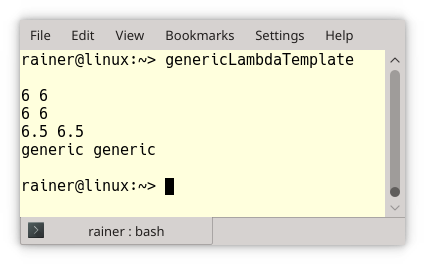
\includegraphics[width=0.6\textwidth]{content/3/chapter4/images/8.png}\\
Use of a generic lambda and a function template
\end{center}

Generic lambdas introduce a new way to define function templates. In my classes, I’m often asked: Can we use auto in functions to get function templates? Not with C++14, but you can with C++20.

In C++20, you can use unconstrained placeholders (auto) or constrained placeholders (concepts) in function declarations to automatically get function templates. The rule for applying is as simple as it could be. In each place where you can use an unconstrained placeholder auto, you can use a concept. I will detail this fully in the section on abbreviated function templates.

\noindent
4.1.5.2\hspace{0.2cm} Placeholders

\noindent
Use of constrained placeholders instead of unconstrained placeholders
\begin{lstlisting}[style=styleCXX]
// placeholders.cpp

#include <concepts>
#include <iostream>
#include <vector>

std::integral auto getIntegral(int val){
	return val;
}

int main(){

std::cout << std::boolalpha << '\n';
	
	std::vector<int> vec{1, 2, 3, 4, 5};
	for (std::integral auto i: vec) std::cout << i << " ";
	std::cout << '\n';
	
	std::integral auto b = true;
	std::cout << b << '\n';
	
	std::integral auto integ = getIntegral(10);
	std::cout << integ << '\n';
	
	auto integ1 = getIntegral(10);
	std::cout << integ1 << '\n';
	
	std::cout << '\n';

}
\end{lstlisting}

The concept std::integral can be used as a return type (line 7), in a range-based for loop (line 16), or as a type for variable b (line 19), or variable integ (line 22). To see the symmetry between auto and concepts, line 25 uses auto alone instead of std::integral auto, which is used on line 22. Hence, integ1 can accept a value of any type.

\begin{tcblisting}{commandshell={}}
1 2 3 4 5
true
10
10
\end{tcblisting}

\begin{center}
Constrained placeholders instead of unconstrained placeholders in action
\end{center}

\subsubsubsection{4.1.6\hspace{0.2cm} Abbreviated Function Templates}

With C++20, you can use an unconstrained placeholder (auto) or a constrained placeholder (concept) in a function declaration and this function declaration automatically becomes a function template.

\noindent
Abbreviated function templates
\begin{lstlisting}[style=styleCXX]
// abbreviatedFunctionTemplates.cpp

#include <concepts>
#include <iostream>

template<typename T>
requires std::integral<T>
T gcd(T a, T b) {
	if( b == 0 ) return a;
	else return gcd(b, a % b);
}

template<typename T>
T gcd1(T a, T b) requires std::integral<T> {
	if( b == 0 ) return a;
	else return gcd1(b, a % b);
}

template<std::integral T>
T gcd2(T a, T b) {
	if( b == 0 ) return a;
	else return gcd2(b, a % b);
}

std::integral auto gcd3(std::integral auto a, std::integral auto b) {
	if( b == 0 ) return a;
	else return gcd3(b, a % b);
}

auto gcd4(auto a, auto b){
	if( b == 0 ) return a;
	return gcd4(b, a % b);
}

int main() {

	std::cout << '\n';
	
	std::cout << "gcd(100, 10)= " << gcd(100, 10) << '\n';
	std::cout << "gcd1(100, 10)= " << gcd1(100, 10) << '\n';
	std::cout << "gcd2(100, 10)= " << gcd2(100, 10) << '\n';
	std::cout << "gcd3(100, 10)= " << gcd3(100, 10) << '\n';
	std::cout << "gcd4(100, 10)= " << gcd4(100, 10) << '\n';
	
	std::cout << '\n';

}
\end{lstlisting}

The definitions of the function templates gcd (line 6), gcd1 (line 13), and gcd2 (line 19) are the ones I already presented in section Four ways to use a concept. gcd uses a requires clause, gcd1 a trailing requires clause and gcd2 a constrained template parameter. Now to something new. Function template gcd3 has the concept std::integral as a type parameter and becomes, therefore, a function template with restricted type parameters. In contrast, gcd4 is equivalent to function templates with no restriction on its type parameters. The syntax used in gcd3 and gcd4 to create a function template is called abbreviated function templates syntax.

\begin{tcblisting}{commandshell={}}
gcd(100, 10)= 10
gcd1(100, 10)= 10
gcd2(100, 10)= 10
gcd3(100, 10)= 10
gcd4(100, 10)= 10
\end{tcblisting}

\begin{center}
Constrained
\end{center}

Let me stress this symmetry by demonstrying it in another example below.

By using auto as a type parameter, the function add becomes a function template and is equivalent to the equally-named function template add.

\noindent
The equivalent function and function template add
\begin{lstlisting}[style=styleCXX]
template<typename T, typename T2>
auto add(T fir, T2 sec) {
	return fir + sec;
}

auto add(auto fir, auto sec) {
	return fir + sec;
}
\end{lstlisting}

Accordingly, due to the usage of the concept std::integral, the function sub is equivalent to the function template sub.

\noindent
The equivalent function and function template sub
\begin{lstlisting}[style=styleCXX]
template<std::integral T, std::integral T2>
std::integral auto sub(T fir, T2 sec) {
	return fir - sec;
}

std::integral auto sub(std::integral auto fir, std::integral auto sec) {
	return fir - sec;
}
\end{lstlisting}

The function and the function template can have arbitrary types. This means both types can be different but must be integral. For example, a call sub(100, 10) and also sub(100, true) would be valid.

There is one interesting feature still missing in the abbreviated function templates syntax: you can overload on auto or concepts.

\noindent
4.1.6.1\hspace{0.2cm} Overloading

The following functions overload are overloaded on auto, on the concept std::integral, and on the type long.

\noindent
Abbreviated function templates and overloading
\begin{lstlisting}[style=styleCXX]
// conceptsOverloading.cpp

#include <concepts>
#include <iostream>

void overload(auto t){
	std::cout << "auto : " << t << '\n';
}

void overload(std::integral auto t){
	std::cout << "Integral : " << t << '\n';
}

void overload(long t){
	std::cout << "long : " << t << '\n';
}

int main(){

	std::cout << '\n';
	
	overload(3.14);
	overload(2010);
	overload(2020L);
	
	std::cout << '\n';

}
\end{lstlisting}

The compiler chooses the overload on auto (line 6) with a double, the overload on the concept std::integral (line 10) with an int, and the overload on long (line 14) with a long.

\begin{tcblisting}{commandshell={}}
auto : 3.14
Integral : 2010
long : 2020
\end{tcblisting}

\begin{center}
Abbreviated function templates and overloading
\end{center}

\begin{tcolorbox}[colback=blue!5!white,colframe=blue!75!black,title={What we don’t get: Template Introduction}]
Maybe you are missing one feature in this chapter on concepts: template introduction. Template introduction was part of the technical specification on concepts, \href{https://www.iso.org/standard/64031.html}{TS ISO/IEC TS 19217:2015}, and was an experimental implementation of concepts. \href{https://en.wikipedia.org/wiki/GNU_Compiler_Collection}{GCC 6} fully implemented the concepts TS. Besides the syntactic differences from concepts in C++20, the concepts TS supported a concise way of defining templates.

In the following example assume that Integral is a concept.

\noindent
Template introduction in the concepts TS
\begin{lstlisting}[style=styleCXX]
Integral{T}
Integral gcd(T a, T b){
	if( b == 0 ){ return a; }
	else{
		return gcd(b, a % b);
	}
}

Integral{T}
class ConstrainedClass{};
\end{lstlisting}

This small code snippet above used template introduction in two ways. First, to define a function template with a constrained template parameter; second, to define a class template with a constrained template parameter. Template introduction had one limitation. You could only use it with a constrained template parameter (concept), but not with an unconstrained template parameter (auto). This asymmetry could easily be overcome by defining a concept that always returns true: 

\noindent
The concept Generic is always fulfilled
\begin{lstlisting}[style=styleCXX]
template<typename T>
concept bool Generic(){
	return true;
}
\end{lstlisting}

Don’t be irritated, I used in the example the concepts TS syntax to define the Generic concept. The C++20 syntax is slightly more concise. Read more details of the C++20 syntax in section Defining Concepts.
\end{tcolorbox}

\subsubsubsection{4.1.7\hspace{0.2cm} Predefined Concepts}

The golden rule “Don’t reinvent the wheel” also applies to concepts. The \href{https://isocpp.github.io/CppCoreGuidelines/CppCoreGuidelines}{C++ Core Guidelines} are very clear about this rule: T.11: Whenever possible, use standard concepts. Consequently, I want to give you an overview of the important predefined concepts. I intentionally ignore any special or auxiliary concepts.

All predefined concepts are detailed in the latest C++20 working draft, \href{https://isocpp.org/files/papers/N4860.pdf}{N4860}, and finding them all can be quite a challenge! Most of the concepts are in chapter 18 (concepts library) and chapter 24 (ranges library). Additionally, a few concepts are in chapter 17 (language support library), chapter 20 (general utilities library), chapter 23 (iterators library), and chapter 26 (numerics library). The C++20 draft N4860 also has an index to all library concepts and shows how the concepts are implemented.

\noindent
4.1.7.1\hspace{0.2cm} Language Support Library

This section discusses an interesting concept, three\_way\_comparable. It is used to support the threeway comparison operator. It is specified in the header <compare>.

More formally, let a and b be values of type T. This values are three\_way\_comparable only if:

\begin{tcblisting}{commandshell={}}
• (a <=> b == 0) == bool(a == b) is true
• (a <=> b != 0) == bool(a != b) is true
• ((a <=> b) <=> 0) and (0 <=> (b <=> a)) are equal
• (a <=> b < 0) == bool(a < b) is true
• (a <=> b > 0) == bool(a > b) is true
• (a <=> b <= 0) == bool(a <= b) is true
• (a <=> b >= 0) == bool(a >= b) is true
\end{tcblisting}

\noindent
4.1.7.2\hspace{0.2cm} Concepts Library

The most frequently used concepts can be found in the concepts library. They are defined in the <concepts> header.

\noindent
4.1.7.2.1\hspace{0.2cm} Language-related concepts

This section has about 15 concepts that should be self-explanatory. These concepts express relationships between types, type classifications, and fundamental type properties. Their implementation is often directly based on the corresponding function from the \href{https://en.cppreference.com/w/cpp/header/type_traits}{type-traits library}. Where deemed necessary, I provide additional explanation.

\begin{itemize}
\item 
same\_as

\item 
derived\_from

\item 
convertible\_to

\item 
common\_reference\_with: common\_reference\_with<T, U> must be well-formed and T and U must be convertible to a reference type C, where C is the same as common\_reference\_t<T, U>

\item 
common\_with: similar to common\_reference\_with, but the common type C is the same as common\_type\_t<T, U> and may not be a reference type

\item 
assignable\_from

\item 
swappable
\end{itemize}

\noindent
4.1.7.2.2\hspace{0.2cm} Arithmetic Concepts

\begin{itemize}
\item 
integral

\item 
signed\_integral

\item 
unsigned\_integral

\item 
floating\_point
\end{itemize}

The standard’s definition of the arithmetic concepts is straightforward:

\begin{lstlisting}[style=styleCXX]
template<class T>
concept integral = is_integral_v<T>;

template<class T>
concept signed_integral = integral<T> && is_signed_v<T>;

template<class T>
concept unsigned_integral = integral<T> && !signed_integral<T>;

template<class T>
concept floating_point = is_floating_point_v<T>;
\end{lstlisting}

\noindent
4.1.7.2.3\hspace{0.2cm} Lifetime Concepts

\begin{itemize}
\item 
destructible

\item 
constructible\_from

\item 
default\_constructible

\item 
move\_constructible

\item 
copy\_constructible
\end{itemize}

\noindent
4.1.7.2.4\hspace{0.2cm} Comparison Concepts

\begin{itemize}
\item 
equality\_comparable

\item 
totally\_ordered
\end{itemize}

Maybe you know it from your mathematics studies: For values a, b, and c of type T, T models totally\_ordered if and only if

\begin{itemize}
\item 
Exactly one of bool(a < b), bool(a > b), or bool(a == b) is true

\item 
If bool(a < b) and bool(b < c), then bool(a < c)

\item 
bool(a > b) == bool(b < a)

\item 
bool(a <= b) == !bool(b < a)

\item 
bool(a >= b) == !bool(a < b)
\end{itemize}

\noindent
4.1.7.2.5\hspace{0.2cm} Object Concepts

\begin{itemize}
\item 
movable

\item 
copyable

\item 
semiregular

\item 
regular
\end{itemize}

Here are the concise definitions of the four concepts:

\begin{lstlisting}[style=styleCXX]
template<class T>
concept movable = is_object_v<T> && move_constructible<T> &&
					assignable_from<T&, T> && swappable<T>;

template<class T>
concept copyable = copy_constructible<T> && movable<T> &&
					assignable_from<T&, T&> &&
					assignable_from<T&, const T&> && assignable_from<T&, const T>;

template<class T>
concept semiregular = copyable<T> && default_initializable<T>;

template<class T>
concept regular = semiregular<T> && equality_comparable<T>;
\end{lstlisting}

I have to add a few words. The concept movable requires for T that is\_object\_v<T> holds. From the definition of the type-trait is\_object<T> this means that T is either a scalar, an array, a union, or a class.

I implement the concept semiregular and regular in the section define concepts. Informally, a semiregular type behaves similar to an int, and a regular type behaves similarly to an int and can be compared using ==.

\noindent
4.1.7.2.6\hspace{0.2cm} Callable Concepts

\begin{itemize}
\item 
invocable

\item 
regular\_invocable: a type models invocable and equality-preserving, and does not modify the function arguments; equality-preserving means the it produces the same output when given the same input

\item 
predicate: a type models a predicate if it models invocable and returns a boolean
\end{itemize}

\noindent
4.1.7.3\hspace{0.2cm} General Utilities Library

This chapter in the standard has only special memory concepts; therefore I don’t refer to them here.

\noindent
4.1.7.4\hspace{0.2cm} Iterators Library

The iterators library has many important concepts. They are defined in the <iterator> header. Here are the iterator categories:

\begin{itemize}
\item 
input\_iterator

\item 
output\_iterator

\item 
forward\_iterator

\item 
bidirectional\_iterator

\item 
random\_access\_iterator

\item 
contiguous\_iterator
\end{itemize}

The six categories of iterators correspond to the respective iterator concepts. The table below provides two interesting pieces of information. For the three most prominent iterator categories, the table shows their properties and the associated standard library containers.

\begin{center}
Properties and Containers of each iterator category
\end{center}

\begin{table}[H]
\centering
\begin{tabular}{lll}
\textbf{Iterator Category}   & \textbf{Properties} & \textbf{Containers}                                                                                     \\ \hline
std::forward\_iterator &
\begin{tabular}[c]{@{}l@{}}++It,It++,*It\\ It==It2, It!=It2\end{tabular} &
\begin{tabular}[c]{@{}l@{}}std::unordered\_set\\ std::unordered\_map\\ std::unordered\_multiset\\ std::unordered\_multimap\\ std::forward\_list\end{tabular} \\
std::bidirectional\_iterator & --It,It--           & \begin{tabular}[c]{@{}l@{}}std::set\\ std::map\\ std::multiset\\ std::multimap\\ std::list\end{tabular} \\
std::random\_access\_iterator &
\begin{tabular}[c]{@{}l@{}}It{[}i{]}\\ It += n, It -= n\\ It + n, It - n,\\ n + It,\\ It - It2,\\ It \textless It2, It \textless{}= It2\\ It \textless It2, It \textgreater{}= It2\end{tabular} &
\begin{tabular}[c]{@{}l@{}}std::array\\ std::vector\\ std::deque\\ std::string\end{tabular}
\end{tabular}
\end{table}

The following relation holds: A random-access-iterator is a bidirectional iterator, and a bidirectional iterator is a forward iterator. A contiguous iterator is a random-access-iterator and requires that the elements of the container are stored contiguously in memory. This means std::array, std::vector, and std::string, but not std::deque, support contiguous iterators.

\noindent
4.1.7.4.1\hspace{0.2cm} Algorithm Concepts

\begin{itemize}
\item 
permutable: in-place reordering of elements is possible

\item 
mergeable: merging sorted sequences into an output sequence is possible

\item 
sortable: permuting a sequence into an ordered sequence is possible
\end{itemize}

\noindent
4.1.7.5\hspace{0.2cm} Ranges Library

The ranges library contains the concepts critical to the ranges and views features. They are similar to the concepts in the iterators library and are defined in the <ranges> header.

\noindent
4.1.7.5.1\hspace{0.2cm} Ranges

\begin{itemize}
\item 
range: A range specifies a group of items that you can iterate over. It provides a begin iterator and an end sentinel. Of course, the containers of the STL are ranges.
\end{itemize}

There are further refinements for std::ranges::range.

\begin{itemize}
\item 
input\_range: specifies a range whose iterator type satisfies input\_iterator (e.g. can iterate from beginning to end at least once)

\item 
output\_range: specifies a range whose iterator type satisfies output\_iterator

\item 
forward\_range: specifies a range whose iterator type satisfies forward\_iterator (can iterate from beginning to end more than once)

\item 
bidirectional\_range : specifies a range whose iterator type satisfies bidirectional\_iterator (can iterate forward and backward more than once)

\item 
random\_access\_range: specifies a range whose iterator type satisfies random\_access\_iterator (can jump in constant time to an arbitrary element with the index operator [])

\item 
contiguous\_range: specifies a range whose iterator type satisfies contiguous\_iterator (elements are stored consecutively in memory)
\end{itemize}

Each container of the Standard Template Library supports a specific range. The supported range specifies the capabilities of its iterators.

\begin{center}
Properties and containers of each range concept
\end{center}

\begin{table}[H]
\centering
\begin{tabular}{lll}
\textbf{Iterator Category}        & \textbf{Properties} & \textbf{Containers}                                                                                     \\ \hline
std::ranges::input\_range &
\begin{tabular}[c]{@{}l@{}}++It,It++,*It\\ It==It2, It!=It2\end{tabular} &
\begin{tabular}[c]{@{}l@{}}std::unordered\_set\\ std::unordered\_map\\ std::unordered\_multiset\\ std::unordered\_multimap\\ std::forward\_list\end{tabular} \\
std::ranges::bidirectional\_range & --It,It--           & \begin{tabular}[c]{@{}l@{}}std::set\\ std::map\\ std::multiset\\ std::multimap\\ std::list\end{tabular} \\
std::ranges::random\_access\_range &
\begin{tabular}[c]{@{}l@{}}It{[}i{]}\\ It += n, It -= n\\ It + n, It - n,\\ n + It,\\ It - It2,\\ It \textless It2, It \textless{}= It2\\ It \textless It2, It \textgreater{}= It2\end{tabular} &
std::deque \\
std::ranges::contiguous\_range &
\begin{tabular}[c]{@{}l@{}}It{[}i{]}\\ It += n, It -= n\\ It + n, It - n,\\ n + It,\\ It - It2,\\ It \textless It2, It \textless{}= It2\\ It \textless It2, It \textgreater{}= It2\end{tabular} &
\begin{tabular}[c]{@{}l@{}}std::array\\ std::vector\\ std::string\end{tabular}
\end{tabular}
\end{table}

A container supporting the std::ranges::contiguous\_range concept, supports all revious mentioned concepts in the table such as std::ranges::random\_access\_range, std::ranges::bidirectional\_range, and std::ranges::input\_range. The same holds for all other ranges.

\noindent
4.1.7.5.2\hspace{0.2cm} Views

A std::ranges::view typically something that you apply on a range and performs some operation. A view does not own data and the time a view takes to copy, move, or assign is constant. Here is a quote from Eric Niebler’s range-v3 implementation, which is the basis for the C++20 ranges: “Views are composable adaptations of ranges where the adaptation happens lazily as the view is iterated.”

\noindent
4.1.7.6\hspace{0.2cm} Numeric Library

The numeric library provides the concept of a uniform\_random\_bit\_generator that is defined in the header <random>. A uniform\_random\_bit\_generator g of type G must return uniformly-distributed unsigned integers. Additionally, a uniform random-bit generator g of type G has to support the member functions G::min and G::max.

\subsubsubsection{4.1.8\hspace{0.2cm} Defining Concepts}

When the concept you are looking for is not one of the predefined concepts in C++20, you must define your own concept. In this section I will define a few concepts which will be distinguishable from the predefined concepts through the use of CamelCase syntax. Consequently, my concept for a signed integral is named SignedIntegral, whereas the C++ standard concept goes by the name signed\_integral.

The syntax for defining a concept is straightforward:

\noindent
Concept definition
\begin{lstlisting}[style=styleCXX]
template <template-parameter-list>
concept concept-name = constraint-expression;
\end{lstlisting}

A concept definition starts with the keyword template and has a template parameter list. The second line is more interesting. It uses the keyword concept followed by the concept name and the constraint expression.

A constraint-expression can either be:

\begin{itemize}
\item 
A logical combination of other concepts or compile-time predicates

\begin{itemize}
\item 
Logical combination can be built out of conjunctions (\&\&), disjunctions (||), or negations (!)

\item 
Compile-time predicates are callables that return a boolean value at compile time
\end{itemize}

\item 
A requires expression
\begin{itemize}
\item 
Simple requirements

\item 
Type requirements

\item 
Compound requirements

\item 
Nested requirements
\end{itemize}
\end{itemize}

In the next two sections I will demonstrate various ways of defining concepts.

\noindent
4.1.8.1\hspace{0.2cm} A Logical Combination of other Concepts and Compile-Time Predicates

You can combine concepts and compile time predicates using conjunctions (\&\&) and disjunctions (||). When building your logical combination, you can negate components by using the exclamation mark (!). Thanks to the many compile-time predicates of the \href{https://en.cppreference.com/w/cpp/header/type_traits}{type-traits library}, you have at your disposal all tools required to build powerful concepts.

\begin{tcolorbox}[colback=red!5!white,colframe=red!75!black,title=Don’t define Concepts Recursively or try to Constrain them]
A recursive definition of a concept is not valid:
	
\noindent
Recursively defining a concept
\begin{lstlisting}[style=styleCXX]
template<typename T>
concept Recursive = Recursive<T*>;
\end{lstlisting}
	
The GCC compiler complains in this case that 'Recursive' was not declared in this scope.

When you try to constrain a concept such as in the following code snippet, the GCC compiler unambiguously complains that a concept cannot be constrained.
	
\noindent
Constraining a concept
\begin{lstlisting}[style=styleCXX]
template<typename T>
concept AlwaysTrue = true;

template<typename T>
requires AlwaysTrue<T>
concept Error = true;
\end{lstlisting}

\end{tcolorbox}

Let’s start with the concepts Integral, SignedIntegral, and UnsignedIntegral.

\noindent
The concepts Integral, SignedIntegral, and UnsignedIntegral
\begin{lstlisting}[style=styleCXX]
template <typename T>
concept Integral = std::is_integral<T>::value;

template <typename T>
concept SignedIntegral = Integral<T> && std::is_signed<T>::value;

template <typename T>
concept UnsignedIntegral = Integral<T> && !SignedIntegral<T>;
\end{lstlisting}

I used the type-traits function \href{https://en.cppreference.com/w/cpp/types/is_integral}{std::is\_integral} to define the concept Integral (line 2). Thanks to the function std::is\_signed, I refine the concepts Integral to the concept SignedIntegral (line 4). Finally, negating the concept SignedIntegral gives me the concept UnsignedIntegral (line 7).

Okay, let’s try it out.

\noindent
Use of the concepts Integral, SignedIntegral, and UnsignedIntegral
\begin{lstlisting}[style=styleCXX]
// SignedUnsignedIntegrals.cpp

#include <iostream>
#include <type_traits>

template <typename T>
concept Integral = std::is_integral<T>::value;

template <typename T>
concept SignedIntegral = Integral<T> && std::is_signed<T>::value;

template <typename T>
concept UnsignedIntegral = Integral<T> && !SignedIntegral<T>;

void func(SignedIntegral auto integ) {
	std::cout << "SignedIntegral: " << integ << '\n';
}

void func(UnsignedIntegral auto integ) {
	std::cout << "UnsignedIntegral: " << integ << '\n';
}

int main() {
	
	std::cout << '\n';
	
	func(-5);
	func(5u);
	
	std::cout << '\n';

}
\end{lstlisting}

I used the abbreviated function-template syntax to overload the function func on the concept SignedIntegral (line 15) and UnsignedIntegral (line 19). The compiler chooses the expected overload:

\begin{tcblisting}{commandshell={}}
SignedIntegral: -5
UnsignedIntegral: 5
\end{tcblisting}

\begin{center}
Use of the concepts SignedIntegral, and UnsignedIntegral
\end{center}

For completeness reasons, the following concept Arithmetic uses disjunction.

\noindent
The concept Arithmetic
\begin{lstlisting}[style=styleCXX]
template <typename T>
concept Arithmetic = std::is_integral<T>::value || std::is_floating_point<T>::value;
\end{lstlisting}

\noindent
4.1.8.2\hspace{0.2cm} Requires Expressions

Thanks to requires expressions, you can define powerful concepts. A requires expression has the following form:

\noindent
Requires expression
\begin{lstlisting}[style=styleCXX]
requires (parameter-list(optional)) {requirement-seq}
\end{lstlisting}

\begin{itemize}
\item 
parameter-list: A comma-separated list of parameters, such as in a function declaration

\item 
requirement-seq: A sequence of requirements, consisting of simple, type, compound, or nested requirements
\end{itemize}

\noindent
4.1.8.2.1\hspace{0.2cm} Simple Requirements

The following concept Addable is a simple requirement:

\noindent
The concept Addable
\begin{lstlisting}[style=styleCXX]
template<typename T>
concept Addable = requires (T a, T b) {
	a + b;
};
\end{lstlisting}

The concept Addable requires that the addition a + b of two values of the same type T is possible.

\begin{tcolorbox}[colback=blue!5!white,colframe=blue!75!black,title=Avoid Anonymous Concepts: requires requires]
	
You can define an anonymous concept and directly use it. Avoid it. This makes your code hard to read and you cannot reuse your concepts.

\noindent
An anonymous concept for adding two concepts
\begin{lstlisting}[style=styleCXX]
template<typename T>
	requires requires (T x) { x + x; }
T add1(T a, T b) { return a + b; }
\end{lstlisting}

The function template defines its concept ad-hoc. add1 uses a requires expression inside a requires clause. The anonymous concept is equivalent to the previously defined concept Addable and so is the following function template add2 using the named concept Addable.

\noindent
Use of the concept Addable
\begin{lstlisting}[style=styleCXX]
template<Addable T>
T add2(T a, T b) { return a + b; }
\end{lstlisting}

Concepts should encapsulate general ideas and give them a self-explanatory name for reuse. They are invaluable for maintaining code. Anonymous concepts read more like syntactic constraints the template parameters.
	
\end{tcolorbox}

\noindent
4.1.8.2.2\hspace{0.2cm} Type Requirements

In a type requirement, you have to use the keyword typename together with a type name.

\noindent
The concept TypeRequirement
\begin{lstlisting}[style=styleCXX]
template<typename T>
concept TypeRequirement = requires {
	typename T::value_type;
	typename Other<T>;
};
\end{lstlisting}

The concept TypeRequirement requires that type T has a nested member value\_type, and that the class template Other can be instantiated with T.

Let’s try this out:

\noindent
Use of the concepts TypeRequirement
\begin{lstlisting}[style=styleCXX]
#include <iostream>
#include <vector>

template <typename>
struct Other;

template <>
struct Other<std::vector<int>> {};

template<typename T>
concept TypeRequirement = requires {
	typename T::value_type;
	typename Other<T>;
};

int main() {

	TypeRequirement auto myVec= std::vector<int>{1, 2, 3};

}
\end{lstlisting}

The expression TypeRequirement auto myVec = std::vector<int>{1, 2, 3} (line 18) is valid. A \href{https://en.cppreference.com/w/cpp/container/vector}{std::vector} has an inner member value\_type (line 12) and the class template Other can be instantiated with std::vector<int> (line 13).

\noindent
4.1.8.2.3\hspace{0.2cm} Compound Requirements

A compound requirement has the form

\noindent
Compound requirement
\begin{lstlisting}[style=styleCXX]
{expression} noexcept(optional) return-type-requirement(optional);
\end{lstlisting}

In addition to a simple requirement, a compound requirement can have a \href{https://en.cppreference.com/w/cpp/language/noexcept_spec}{noexcept specifier} and a requirement on its return type.

The concept Equal, demonstrated in the following example, uses compound requirements.

\noindent
Definition and use of the concept Equal
\begin{lstlisting}[style=styleCXX]
// conceptsDefinitionEqual.cpp

#include <concepts>
#include <iostream>

template<typename T>
concept Equal = requires(T a, T b) {
	{ a == b } -> std::convertible_to<bool>;
	{ a != b } -> std::convertible_to<bool>;
};

bool areEqual(Equal auto a, Equal auto b){
	return a == b;
}

struct WithoutEqual{
	bool operator==(const WithoutEqual& other) = delete;
};

struct WithoutUnequal{
	bool operator!=(const WithoutUnequal& other) = delete;
};

int main() {

	std::cout << std::boolalpha << '\n';
	std::cout << "areEqual(1, 5): " << areEqual(1, 5) << '\n';
	
	/*
	
	bool res = areEqual(WithoutEqual(), WithoutEqual());
	bool res2 = areEqual(WithoutUnequal(), WithoutUnequal());
	
	*/
	
	std::cout << '\n';

}
\end{lstlisting}

The concept Equal (line 6) requires that its type parameter T supports the equal and not-equal operator. Additionally, both operators have to return a value that is convertible to a boolean. Of course, int supports the concept Equal, but this does not hold for the types WithoutEqual (line 16) and WithoutUnequal (line 20). Consequently, when I use the type WithoutEqual (line 31), I get the following error message when using the GCC compiler.

\begin{center}
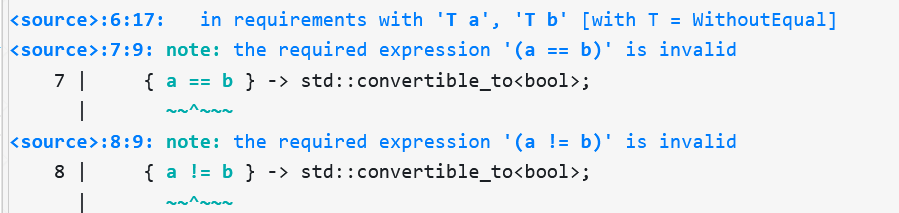
\includegraphics[width=0.8\textwidth]{content/3/chapter4/images/1-4.png}\\
WithoutEqual does not fulfill the concept Equal
\end{center}

\noindent
4.1.8.2.4\hspace{0.2cm} Nested Requirements

A nested requirement has the form

\noindent
Nested requirement
\begin{lstlisting}[style=styleCXX]
requires constraint-expression;
\end{lstlisting}

Nested requirements are used to specify requirements on type parameters.

Here is another way to define the concept UnsignedIntegral (see logical combinations of concepts and predicates):

\noindent
The concepts Integral, SignedIntegral, and UnsignedIntegral
\begin{lstlisting}[style=styleCXX]
// nestedRequirements.cpp

#include <type_traits>

template <typename T>
concept Integral = std::is_integral<T>::value;

template <typename T>
concept SignedIntegral = Integral<T> && std::is_signed<T>::value;

// template <typename T>
// concept UnsignedIntegral = Integral<T> && !SignedIntegral<T>;

template <typename T>
concept UnsignedIntegral = Integral<T> &&
requires(T) {
	requires !SignedIntegral<T>;
};

int main() {

	UnsignedIntegral auto n = 5u; // works
	// UnsignedIntegral auto m = 5; // compile time error, 5 is a signed literal

}
\end{lstlisting}

Line 14 uses with the concept SignedIntegral a nested requirement to refine the concept Integral. Honestly, the commented-out concept UnsignedIntegral in line 11 is more convenient to read.

The concept Ordering in the following section demonstrates the use of nested requirements.

\subsubsubsection{4.1.9\hspace{0.2cm} Application}

In the previous sections I answered two essential questions about concepts: “How can a concept be used?” and “How can you define your concepts?”. In this section, I want to apply the theoretical knowledge provided in those sections to define more advanced concepts such as Ordering, SemiRegular, and Regular.

\noindent
4.1.9.1\hspace{0.2cm} The Concepts Equal and Ordering

I presented already in the short detour to the long, long history of concepts a part of Haskell’s type classes hierarchy:

\begin{center}
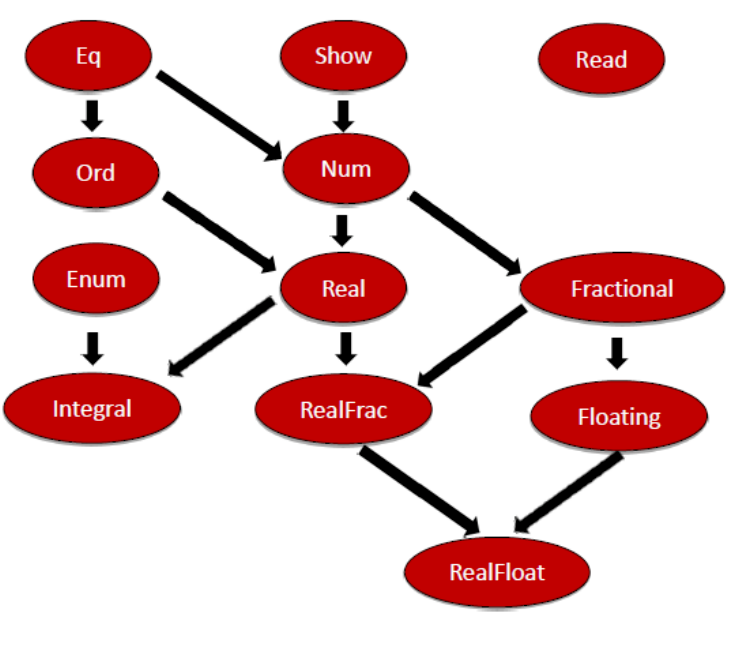
\includegraphics[width=0.8\textwidth]{content/3/chapter4/images/9.png}\\
Haskell Type Classes Hierarchy
\end{center}

The class hierarchy shows that the type class Ord is a refinement of the type class Eq. Haskell expresses this elegantly.

\noindent
A part of Haskell’s type classes hierarchy
\begin{lstlisting}[style=styleCXX]
class Eq a where
	(==) :: a -> a -> Bool
	(/=) :: a -> a -> Bool

class Eq a => Ord a where
	compare :: a -> a -> Ordering
	(<) :: a -> a -> Bool
	(<=) :: a -> a -> Bool
	(>) :: a -> a -> Bool
	(>=) :: a -> a -> Bool
	max :: a -> a -> a
\end{lstlisting}

Each type a supporting the type class Eq (line 1), has to support equality (line 2) and inequality (line 3). Now to the interesting part of this definition. Each type a supporting the type class Ord has to support the type class Eq (class Eq a => Ord a in line 5). Additionally, type a has to support the four comparison operators and the functions compare and max (lines 6 - 11).

Here is my challenge. Can we express Haskell’s relationship between the type classes Eq and Ord with concepts in C++20? For simplicity, I ignore Haskell’s functions compare and max.

\noindent
4.1.9.1.1\hspace{0.2cm} The Concept Ordering

Thanks to the requires expression, the definition of the concept Ordering looks quite similar to the definition of the type class ord in Haskell.

\noindent
The concept Ordering
\begin{lstlisting}[style=styleCXX]
template <typename T>
concept Ordering =
	Equal<T> &&
	requires(T a, T b) {
		{ a <= b } -> std::convertible_to<bool>;
		{ a < b } -> std::convertible_to<bool>;
		{ a > b } -> std::convertible_to<bool>;
		{ a >= b } -> std::convertible_to<bool>;
	};
\end{lstlisting}

The Ordering concept uses nested requirements under the hood. A type T supports the concept Ordering if it supports the concept Equal and, additionally, the four comparison operators. Let’s try it out.

\noindent
Definition and usage of the concept Ordering
\begin{lstlisting}[style=styleCXX]
// conceptsDefinitionOrdering.cpp

#include <concepts>
#include <iostream>
#include <unordered_set>

template<typename T>
concept Equal =
	requires(T a, T b) {
		{ a == b } -> std::convertible_to<bool>;
		{ a != b } -> std::convertible_to<bool>;
	};


template <typename T>
concept Ordering =
	Equal<T> &&
	requires(T a, T b) {
		{ a <= b } -> std::convertible_to<bool>;
		{ a < b } -> std::convertible_to<bool>;
		{ a > b } -> std::convertible_to<bool>;
		{ a >= b } -> std::convertible_to<bool>;
	};

template <Equal T>
bool areEqual(const T& a, const T& b) {
	return a == b;
}

template <Ordering T>
T getSmaller(const T& a, const T& b) {
	return (a < b) ? a : b;
}

int main() {

	std::cout << std::boolalpha << '\n';
	
	std::cout << "areEqual(1, 5): " << areEqual(1, 5) << '\n';
	
	std::cout << "getSmaller(1, 5): " << getSmaller(1, 5) << '\n';
	
	std::unordered_set<int> firSet{1, 2, 3, 4, 5};
	std::unordered_set<int> secSet{5, 4, 3, 2, 1};
	
	std::cout << "areEqual(firSet, secSet): " << areEqual(firSet, secSet) << '\n';
	
	// auto smallerSet = getSmaller(firSet, secSet);
	
	std::cout << '\n';

}
\end{lstlisting}

The function template areEqual (line 25) requires that both arguments a and b have the same type and support the concept Equal. Additionally, the function template getSmaller (line 30) requires that both arguments support the concept Ordering. Of course, integrals such as 1 and 5 support both concepts. A \href{https://en.cppreference.com/w/cpp/container/unordered_set}{std::unordered\_set}, as its name implies, does not fulfill the concept Ordering.

Consequently, I commented out line 48.

\begin{tcblisting}{commandshell={}}
areEqual(1, 5): false
getSmaller(1, 5): 1
areEqual(firSet, secSet): true
\end{tcblisting}

\begin{center}
Use of the concept Ordering
\end{center}

Let’s look at the more interesting case now. What happens, when we compile line 48: auto smallerSet = getSmaller(firSet, secSet);? The GCC compiler complains unambiguously that a std::unordered\_set is not a valid argument for the function template getSmaller.

\begin{center}
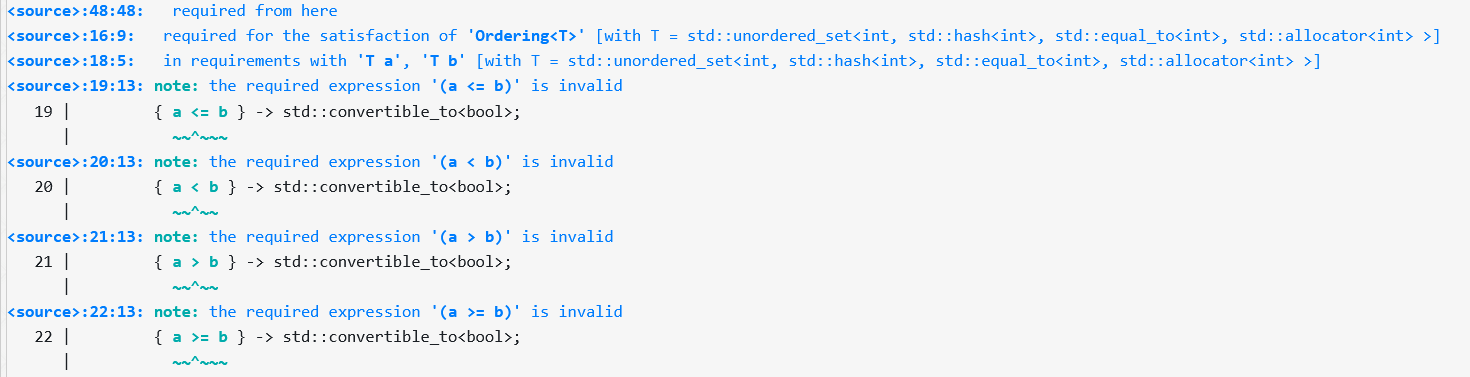
\includegraphics[width=0.8\textwidth]{content/3/chapter4/images/1-5.png}\\
Erroneous usage of the function template getSmaller
\end{center}

The Ordering concept is already part of the C++20 standard.

\begin{itemize}
\item 
std::three\_way\_comparable: is equivalent to the concept Ordering presented above

\item 
std::three\_way\_comparable\_with: allows the comparison of values of different types; e.g.: 1.0 < 1.0f
\end{itemize}

With C++20, we get the three-way comparison operator, also known as the spaceship operator <=>. I present it in full depth in the three-way comparison operator chapter.

\noindent
4.1.9.2\hspace{0.2cm} The Concepts SemiRegular and Regular

When you want to define a concrete type that works well in the C++ ecosystem, you should define a type that “behaves like an int”. Formally, your concrete type should be a regular type. In this section, I define the concepts SemiRegular and Regular.

SemiRegular and Regular are essential ideas in C++. Sorry, I should say concepts. For example, here is rule \href{http://isocpp.github.io/CppCoreGuidelines/CppCoreGuidelines#Rt-regular}{T.46 from the C++ Core Guidelines: T.46: Require template arguments to be at least Regular or SemiRegular}. Now, only one important question is left to answer: What are Regular or SemiRegular types? Before I dive into the details, this is the informal answer:

\begin{itemize}
\item 
A regular type “behaves like an int.” It can be copied and the result of the copy operation is independent of the original one and has the same value.
\end{itemize}

Okay, let me be more formal. A regular type is also a semiregular type, so let’s begin.


\begin{tcolorbox}[colback=blue!5!white,colframe=blue!75!black,title=Regular Types]

\href{https://en.wikipedia.org/wiki/Alexander_Stepanov}{Alexander Stepanov}, the designer of the Standard Template Library, defined the terms regular type and semiregular type. A type, according to him, is regular if it supports these functions

\begin{itemize}
\item 
Copy construction

\item 
Assignment

\item 
Equality

\item 
Destruction

\item 
Total ordering
\end{itemize}

Copy construction implies default construction and Equality implies Inequality. When Stepanov defined the requirements above, move semantics was not present in C++. The book \href{http://elementsofprogramming.com/}{Elements of Programming}, which Alexander Stepanov wrote together with \href{https://www.mcjones.org/paul/}{Paul McJones}, is devoted to regular types.

\end{tcolorbox}

\noindent
4.1.9.2.1\hspace{0.2cm} The Concept SemiRegular

A semiregular type X has to support the Big Six and has to be swappable. The Big Six consists of the following functions:

\begin{itemize}
\item 
Default constructor: X()

\item 
Copy constructor: X(const X\&)

\item 
Copy assignment: X\& operator = (const X\&)

\item 
Move constructor: X(X\&\&)

\item 
Move assignment: X\& operator = (X\&\&)

\item 
Destructor: ∼X()
\end{itemize}

Additionally, X has to be swappable: swap(X\&, X\&)

Thanks to the \href{https://en.cppreference.com/w/cpp/header/type_traits}{type-traits library}, defining the corresponding concept is a no-brainer. First, I define the type trait isSemiRegular and then use it to define the concept SemiRegular.

\begin{lstlisting}[style=styleCXX]
template<typename T>
struct isSemiRegular: std::integral_constant<bool,
								std::is_default_constructible<T>::value &&
								std::is_copy_constructible<T>::value &&
								std::is_copy_assignable<T>::value &&
								std::is_move_constructible<T>::value &&
								std::is_move_assignable<T>::value &&
								std::is_destructible<T>::value &&
								std::is_swappable<T>::value >{};


template<typename T>
concept SemiRegular = isSemiRegular<T>::value;
\end{lstlisting}

The type trait isSemiRegular (line 1) is fulfilled when all type traits to the Big Six (lines 3 - 8) and the type trait std::is\_swappable (line 9) are fulfilled. The remaining step to define the concept SemiRegular is to use the type traits isSemiRegular (line 13).

Let’s continue with the concept Regular.

\noindent
4.1.9.2.2\hspace{0.2cm} The Concept Regular

There is only one step and we are done with defining the concept Regular. In addition to the requirements of the concept SemiRegular, the concept Regular requires that the type is equally comparable. I already defined the Equal concept in the section on requires expressions. Consequently, you are already done. You only have to conjunct the concepts Equal and SemiRegular.

\noindent
Definition of the concept Regular
\begin{lstlisting}[style=styleCXX]
template<typename T>
concept Regular = Equal<T> &&
					SemiRegular<T>;
\end{lstlisting}

Now, I’m curious. How can we define the corresponding concepts std::semiregular and std::regular in C++20?

\noindent
4.1.9.2.3\hspace{0.2cm} std::semiregular and std::regular

C++20 combines the concepts std::semiregular and std::regular using of existing type traits and concepts.

\noindent
Definition of the concept std::semiregular and std::regular
\begin{lstlisting}[style=styleCXX]
template<class T>
concept movable = is_object_v<T> && move_constructible<T> &&
					assignable_from<T&, T> && swappable<T>;

template<class T>
concept copyable = copy_constructible<T> && movable<T> &&
					assignable_from<T&, T&> &&
					assignable_from<T&, const T&> && assignable_from<T&, const T>;

template<class T>
concept semiregular = copyable<T> && default_initializable<T>;

template<class T>
concept regular = semiregular<T> && equality_comparable<T>;
\end{lstlisting}

Interestingly, the std::regular concept is defined similarly to concept Regular. On the other hand, the std::semiregular concept is combined with more elementary concepts, such as std::copyable and std::moveable. The concept std::movable is based on the type-traits function \href{https://en.cppreference.com/w/cpp/types/is_object}{std::is\_object}. cppreference.com also provides a possible implementation of the compile-time predicate.

\noindent
A possible implementation of the type trait std::is\_object
\begin{lstlisting}[style=styleCXX]
template< class T>
struct is_object : std::integral_constant<bool,
					std::is_scalar<T>::value ||
					std::is_array<T>::value ||
					std::is_union<T>::value ||
					std::is_class<T>::value> {};
\end{lstlisting}

A type is an object if it is either a scalar, an array, a union, or a class.

To conclude this section, I want to apply the user-defined concept Regular and the C++20 concept std::regular. The program regularSemiRegular.cpp does this job.

\noindent
Application of the concepts Regular and SemiRegular
\begin{lstlisting}[style=styleCXX]
// regularSemiRegular.cpp

#include <concepts>
#include <vector>
#include <type_traits>

template<typename T>
struct isSemiRegular: std::integral_constant<bool,
		std::is_default_constructible<T>::value &&
		std::is_copy_constructible<T>::value &&
		std::is_copy_assignable<T>::value &&
		std::is_move_constructible<T>::value &&
		std::is_move_assignable<T>::value &&
		std::is_destructible<T>::value &&
		std::is_swappable<T>::value >{};

template<typename T>
concept SemiRegular = isSemiRegular<T>::value;

template<typename T>
concept Equal =
	requires(T a, T b) {
		{ a == b } -> std::convertible_to<bool>;
		{ a != b } -> std::convertible_to<bool>;
};

template<typename T>
concept Regular = Equal<T> &&
				SemiRegular<T>;
				
template <Regular T>
void behavesLikeAnInt(T) {
	// ...
}

template <std::regular T>
void behavesLikeAnInt2(T) {
	// ...
}

struct EqualityComparable { };
bool operator == (EqualityComparable const&,
				  EqualityComparable const&) {
	return true;
}

struct NotEqualityComparable { };

int main() {

	int myInt{};
	behavesLikeAnInt(myInt);
	behavesLikeAnInt2(myInt);
	
	std::vector<int> myVec{};
	behavesLikeAnInt(myVec);
	behavesLikeAnInt2(myVec);
	
	EqualityComparable equComp;
	behavesLikeAnInt(equComp);
	behavesLikeAnInt2(equComp);
	
	NotEqualityComparable notEquComp;
	behavesLikeAnInt(notEquComp);
	behavesLikeAnInt2(notEquComp);

}
\end{lstlisting}

I put all pieces from the previous code-snippets together to define the concept Regular (line 27). The function templates behavesLikeAnInt (line 31) and behavesLikeAnInt2 (line 36) check if the arguments “behave like an int.” This means the user-defined concept Regular and the C++20 concept std::regular are used to establish the condition. As the name suggests, the type EqualityComparable (line 41) supports equality, but the type NotEqualityComparable (line 47) does not. The use of the type NotEqualityComparable in both function calls (lines 64 and 65) is the most interesting part of the program.

Although I’m in the early stage of concepts implementation, I want to compare the error messages of a new GCC and MSVC compilers.

\begin{itemize}
\item 
GCC
\end{itemize}

I used the current GCC 10.2 with the command line argument -std=c++20 on \href{https://godbolt.org/}{Compiler Explorer}. These are essentially the error messages when I use the user-defined concept Regular (line 64):

\begin{center}
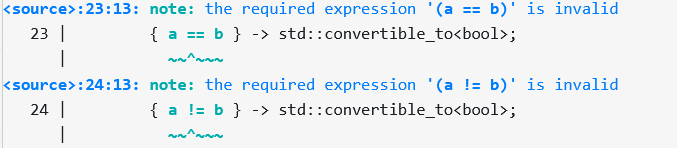
\includegraphics[width=0.8\textwidth]{content/3/chapter4/images/1-6.png}\\
Error message when using the concept Regular
\end{center}

The C++20 concept std::regular is more comprehensive. Consequently, the call in line 65 gives a more comprehensive error message:

\begin{center}
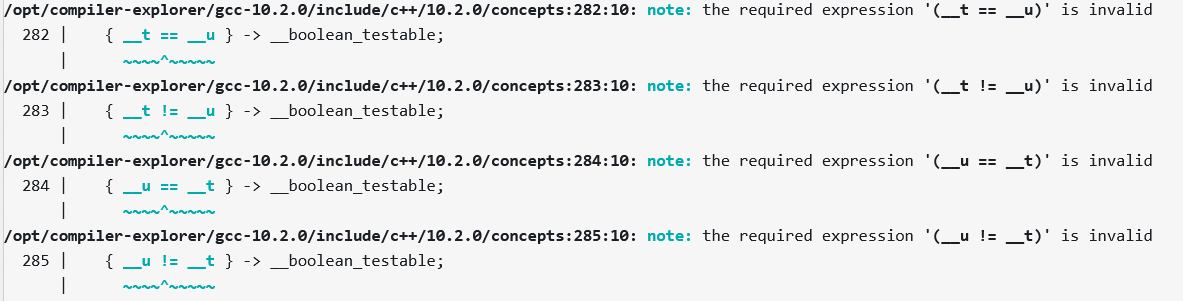
\includegraphics[width=0.8\textwidth]{content/3/chapter4/images/1-7.png}\\
Error message when using the concept std::regular
\end{center}

\begin{itemize}
\item 
MSVC
\end{itemize}

The error message given by the MSVC compiler is too unspecific.

\begin{center}
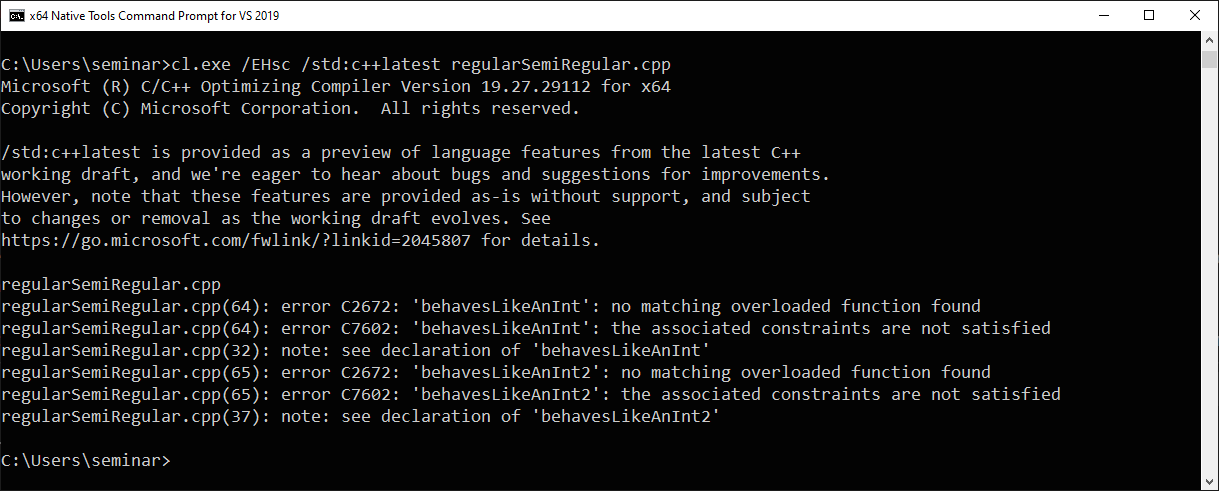
\includegraphics[width=0.8\textwidth]{content/3/chapter4/images/10.png}\\
Error message when using the concepts Regular and std::regular
\end{center}

As you can see from the screenshot, I applied version 19.27.29112 for x64 with the command line /EHSC /std:c++latest.

\begin{tcolorbox}[colback=blue!5!white,colframe=blue!75!black,title=Regular Types]

This small detour expresses my opinion. First, I present the facts, then I draw my conclusion. The facts are based on what has been presented in this chapter. So which arguments speak for evolution or for revolution?

\noindent
\textbf{Evolution}

\begin{itemize}
\item 
Concepts promote working with generic code at a higher level of abstraction.

\item 
Concepts give you understandable error messages when compiling a template fails. They provide nothing you could not achieve with the \href{https://en.cppreference.com/w/cpp/header/type_traits}{type-traits library}, \href{https://en.cppreference.com/w/cpp/language/sfinae}{SFINAE}, and \href{https://en.cppreference.com/w/cpp/language/static_assert}{static\_assert}.

\item 
auto is a kind of unconstrained placeholder. With C++20, we can use concepts as constrained placeholders.

\item 
With C++14, we could use generic lambdas as a convenient way to define function templates.
\end{itemize}

\noindent
\textbf{Revolution}

\begin{itemize}
\item 
Concepts promote working with generic code at a higher level of abstraction.

\item 
Concepts allow us, for the first time, to verify template requirements. Of course, you can also achieve the verification of template parameters with a combination of \href{https://en.cppreference.com/w/cpp/header/type_traits}{type-traits library}, \href{https://en.cppreference.com/w/cpp/language/sfinae}{SFINAE}, and \href{https://en.cppreference.com/w/cpp/language/static_assert}{static\_assert}, but this technique is way too advanced to regard it as a general solution.

\item 
Thanks to the abbreviated function-templates syntax, defining templates has been radically improved.

\item 
Concepts represent semantic categories, but not syntactic constraints. Instead of a concept such as Addable, which requires that a type supports the + operator, we should think in terms of a concept Number, where Number is a semantic category such as Equal or Ordering.
\end{itemize}

\noindent
\textbf{My Conclusion}

There are many arguments whether concepts are an evolutionary step or a revolutionary jump. Mainly because of the semantic categories, I’m on the revolution side. Concepts such as Number, Equality, or Ordering remind me of \href{https://en.wikipedia.org/wiki/Plato}{Plato’s} world of ideas. It is revolutionary that we can now reason about programming in such categories.
\end{tcolorbox}

\begin{tcolorbox}[colback=mygreen!5!white,colframe=mygreen!75!black,title=Distilled Information]
\begin{itemize}
\item 
Functions or classes defined on a specific type or a type parameter have their set of problems. Concepts overcome these problems by putting semantic constraints on type parameters.

\item 
Concepts can be applied in requires clauses, in trailing requires clauses, as constrained template parameters, or in the abbreviated function templates.

\item 
Concept are compile-time predicates that can be used for all kinds of templates. You can overload on concepts, specialize templates on concepts, use concepts for member functions or variadic templates.

\item 
Thanks to C++20 and concepts, the use of unconstrained placeholders (auto) and constrained placeholders (concepts) is unified. Whenever you use auto, you can use concepts in C++20.

\item 
Thanks to the new abbreviated function-templates syntax, defining a function template has become a piece of cake.

\item 
Don’t reinvent the wheel. Before you define your own concepts, study the rich set of predefined concepts in the C++20 standard. When you define your concepts, you can apply two techniques: combine concepts and compile-time predicates or use requires expressions.
\end{itemize}
\end{tcolorbox}



















